\documentclass[a4paper,10pt,onecolumn,preprint,3p]{elsarticle}
% The format for draft in Elsevier is one column. ;D

\usepackage{graphics,subfigure}
\usepackage{amssymb}
\usepackage{amsmath}
\usepackage[dvips]{epsfig}
\usepackage[latin1]{inputenc}
\usepackage{url}
\usepackage{multirow}

\def\CC{{C\hspace{-.05em}\raisebox{.4ex}{\tiny\bf ++}}~}
\addtolength{\textfloatsep}{-0.5cm}
\addtolength{\intextsep}{-0.5cm}

\journal{Journal of XXXXXXXXX}

\begin{document}

\begin{frontmatter}

%%%%%%%%%%%%%%%% Title %%%%%%%%%%%%%%%
\title{Predicting Sales Level for Newly Published Books \\
using Cost-Sensitive Ensemble Methods}


%%%%%%%%%%%%%%%% Authors %%%%%%%%%%%%%%
\author[abd]{Hossam Faris}
\ead{hossam.faris@ju.edu.jo}
\author[ugratc]{Antonio M. Mora}
\ead{amorag@ugr.es}
\author[ugratc]{Pedro A. Castillo}
\ead{pacv@ugr.es}
\author[ugratc]{J.J. Merelo}
\ead{jmerelo@geneura.ugr.es}


\address[abd]{Business Information Technology Department, King Abdullah II School for Information Technology \\
The University of Jordan, Amman, Jordan}
%\address[ugratc]{Department of Signal Theory, Telematics and Communications, ETSIIT and CITIC \\
%University of Granada, Granada, Spain}
\address[ugratc]{Department of Computer Architecture and Computer Technology, ETSIIT and CITIC \\
University of Granada, Granada, Spain}

%\maketitle

%%%%%%%%%%%%%%%%%%%%%%%%%%%%%%%%%%%%%%%%%%%%%%%%%%%%%%%%%%%%%
\begin{abstract}
%First you have to explain why it is enough to predict the level of
%sales, and not the precise number. 
% Antonio - it is true, but how can we justify this, JJ?
% I guess that precision is relative in this kind of methods, since the publisher is not going to print exactly '237' books due to it is the output of a regression method. Instead, there could be a range of books to be printed (as a standard) related with an expected 'low', 'medium', 'high' or 'very high' amount of sales.
% Moreover, I guess that the classification output, considering four classes would work better (more precisely and close to reality) than regression.
% What do you think?
An important task when publishing a new book is determining the number 
of copies to be printed, since doing both a (dramatic) under- or overestimation will lead to important financial losses.
In this paper, we transform this problem into a classification one, defining different sales levels i.e. classes. 
The obtained results will be easier to interpret by publishers than other black-box techniques, 
so these methods can be used as reliable decision-aid tools for publishers, to be considered in their decision as a part of the final stages of the editorial process.
% paragraphs in the abstract is not a good idea.
The problem of predicting these levels has been addressed applying cost-sensitive ensemble methods.
% Antonio - explain briefly what are them  and  the followed methodology.
In order to do so, a real dataset collected by a Spanish publishing company, including the complete sales data for books published in Spain across several years, has been used to design and evaluate the prediction models.
% Explain also the method you are using and why it's an improvement over the previous one - JJ
Results show that %\emph{EXPLAIN THE RESULTS OBTAINED}.

\end{abstract}


\begin{keyword}
% Antonio - to refine later
Book sales forecasting \sep Decision-aid models \sep Feature selection
\sep Classification \sep Ensemble methods %why commas _and_ CAPS? - JJ
\end{keyword}

\end{frontmatter}



%*******************************************************************************
%		            INTRODUCTION
%*******************************************************************************
\section{Introduction}
\label{sec:intro}

% You have to
% 1. Explain the problem: predicting the sales level. 
% 2. Briefly state what has been done so far (previous paper) and how
% this improves over that paper. You will have to compare results,
% too.
% 3. Talk about the methodology and why we think this should give us
% better results.
% 4. Hint at how we are going to prove it.

Reliable sales prediction can enhance the whole production process for different 
companies involved in manufacturing, marketing and trading.
Moreover, in some real-world cases, such as consumer electronics, fashion products and books, new products are presented/launched every season; thus, accurate sales forecasting models could help in marketing campaigns for instance.

Specifically, focusing in the publishing process of a new book, deciding the optimal {\em  print run}, i.e. the number of copies to be printed and delivered to bookstores, is a very challenging problem. Thus, it is extremely
important to develop accurate predictive models which could forecast
the future sales a new book will achieve, in order to optimise
production schedules \cite{Fildes2010,Saeed2008,Zhao2001}, to improve the publishing company profits and to minimise losses, due both to the excess or to the scarcity of units. 
%I would eliminate this paragraph. We have it on the other one.
%Since, according to the results reported in \cite{Fildes2010,Saeed2008}, reducing the error in estimated sales leads to an enhancement of the whole production process.
% Antonio - I agree. Removed

Traditionally the prediction of book sales has been generally based on experts' experience. They analyse data about sales and, taking into account their knowledge of the industry, the production issues, and their perception about trends, take decisions on the production and publication processes.
However, this procedure might be tedious, especially when the amount of data is 
quite large. Moreover, the results are not robust, since different experts could come to different predictions from the same dataset \cite{Sanders1994}.

% TODO: UNDER CONSTRUCTION
% Define level of sales before you use it here. Is it the actual
% number? A ballpark? If it's the actual number, it should be unit
% sales - JJ 
% Antonio - done in a paragraph below
It is also possible to use any kind of decision-aid tool, such as estimating or predictive models. These should be able to compute an accurate number of expected sales which can help the publisher (expert) to take the optimal decision. 
Thus, in our previous work \cite{Castillo2016books}, the main factors influencing sales where analyzed in order to create that kind of tool.
In that paper, several regression methods were applied to estimate sales for new launched books using a real dataset of book sales related to the Spanish market, provided by the Spanish publishing company Trevenque Editorial S.L.\footnote{\tt http://editorial.trevenque.es}.

% Antonio - this is themotivation/justification of the present work. Please all chek it. ;D
However, the complexity of those models, even if they yielded a decision tree might be a flaw for publishers when they must work with them in real scenarios, since the leaves of those trees are complicated regression formulae.
In addition, the estimated number despite being accurate according to the experiments, might not be very reliable for these experts, in the sense that most of them would prefer to deal with categorical variables to include in their own `prediction formulae'.

Thus, having in mind `the human factor' of the print-run decision process, in this paper we have addressed the problem from a new perspective. We have defined, with the help of an expert, different \textit{levels or ranges of sales}, composing different incremental categories: \textit{Low, Medium, High} and \textit{Very High}. Then, these have been considered as classes, so the given dataset has been labelled according to them, and the problem has been faced as a classification one.

Moreover, handling the problem as a classification task let us to
emphasize on the ranges which could be more `critical', e.g. the most
profitable books (High and Very High categories). % You have used
                                % italics for this before but no
                                % emphasis now. You have to unify
                                % typography - JJ
Thus, we can penalize more the misclassification of these categories and, consequently, this tool will perform a better identification of successful books than our previous approach \cite{Castillo2016books}.
% which will be definitely very interesting for publishers.

In order to solve this problem, in this work we propose configuring complex models based on ensembles \cite{Qiu2014} in order to determine the actual level of sales a new book will achieve.
% Antonio - justify why ensembles have been chosen instead of other classification approaches: accuracy, perform, easier to interpret, faster, ...
Another advantage of the proposed approach is that they are easier to interpret than `black box' forecasting methods, such as regression techniques. So, using these ensemble methods, publishers will be able to combine their expert knowledge about the 
market with the obtained models in order to get a reliable estimation 
on book sales level. Moreover, as the output will be just a class, they will be able to understand and justify better their decision.

% Antonio: TODO - explain how are we going to demonstrate the value of this proposal and how are we going to prove that it is better than our previous approach... Will it 'better' or just 'different' and also valid as a decision tool? Will we count with an expert to compare them? Maybe JJ could be the Expert? :D

% Antonio: TODO - rewrite with the final structure
The rest of this paper is structured as follows: 
A detailed review of the approaches related to sales prediction in similar scopes is presented in Section \ref{sec:soa}.
Then, Section \ref{sec:methodology} details the methodology considered in the present study. 
Obtained results after extensive experimentation are presented in Section \ref{sec:experiments_results}.
Finally, conclusions and future lines of work are presented in Section \ref{sec:conclusions_future_work}.


%*******************************************************************************
%										STATE OF THE ART
%*******************************************************************************
\section{State of the art on sales forecasting} 
\label{sec:soa}

%Sales prediction is an important problem that can improve the quality of business strategy for different companies. 
% Antonio - not needed to mention this again in this section. Maybe we can move it to the introduction. ;)
Traditionally, sales prediction problems have been solved using advanced mathematical and machine learning-based methods
% Antonio - why are they 'advanced'?
such as regression models \cite{Papalexopoulos1990}, neural networks \cite{Yoo1999}, fuzzy systems \cite{Mastorocostas2001}, or mixture of methods \cite{Chang2006715,Meulstee2008,ChiJie2012}.

In this line of work, the most widely used techniques to tackle sales forecasting problems have been time-series prediction
\cite{Chu2003,Brown1959,Winters1960,Box1969,Papalexopoulos1990}. %,KayacanUK10}. % Antonio - the last reference doesn't exist
However these methods are strongly dependent on problem data, so the obtained predictions are highly affected by their correctness.
Moreover, this kind of methods are based on using historical data about an article to make time series. However, in the case of new products sales prediction (such as the issue of new books), there is no available historical sales data for that product \cite{ChingChin2010}, and only pre-sales data can be considered \cite{FaderHardie2005,Madsen2008}, 
i.e. variables known before the product is on sale. 

Not only the lack of historical data makes this a complex problem, but also the fact that several `external' variables (seasonality, promotions, or fashions) might influence predictions
\cite{Lapide1999,Thomassey2012,Xia2012,SThomassey2014,ChernWSF15}.
% Antonio - choose just a couple of references to justify this. ;)

Due to the difficulty this problem represents when forecasting sales of new 
products, some authors have proposed using different data mining methods, such as data clustering and fuzzy neural networks \cite{Chang2009} or extreme learning machine (ELM) - a feedforward neural network in which the weights are just computed once and not changed - with adaptive metrics of inputs \cite{Xia2012}.

In this line, several authors have applied the \textit{ensemble} (or combination) of models for sales forecasting, as it is done in \cite{ChiJie2012}, where a hybrid forecasting method integrates ensemble empirical model decomposition and ELM to develop an effective forecasting model for computer products sales.
Also, Meulstee et al. \cite{Meulstee2008} developed an ensemble learning approach for better handling of seasonal changes and fluctuations in consumer demands, whereas Chang et al. \cite{Chang2006715} integrated a fuzzy logic controller and an artificial neural network for sales forecasting in printed circuit board industry.

Other authors have faced the problem of sales forecasting in textile-apparel 
fashion industry - a very similar issue to the new book publishing problem - 
using a clustering method together with decision trees, as in \cite{SThomassey2014}, or a forecasting method based on ELM with adaptive metrics of inputs \cite{Xia2012}.
% Antonio - comment this last paper

Ching et al. \cite{ChingChin2010} used a decision-support system to classify new 
products (tea, cosmetics and soft drink) based on their sales patterns, assuming 
that products in the same class would follow a similar sales pattern. 
In any case, the proposed system can not deal with qualitative data related to the products. 
In this paper, however, several classification-based approaches have been implemented and tested, also considering categorical data.


%Finally, in those problems where historical data are available, authors have 
%proposed to apply classical time series forecasting methods.
% Antonio - we said previously more or less that Time Series Prediction is not recommended

In \cite{Chang2009} a hybrid model integrating K-Means and fuzzy neural networks 
to forecast the future sales of a printed circuit board is proposed.
% Antonio - compare it with our work
Recent works propose to take advantage of the information extracted from online reviews, such as in \cite{ChernWSF15} where it is conducted an analysis on historical data throughout online reviews, reviewer characteristics, and review influences; in order to understand how electronic `word-of-mouth' influences product sales.
Similar research efforts took advantage of the information published
on specialized  %please revise 
blogs \cite{Moon2010ICSSSM,Moon2010ICEC}, confirming there is a relationship between the number of blog references and the book sales. Therefore, different sales patterns have been observed by analysing books in series, i.e. the first book published takes the longest period to achieve every single sales scale, while the second book takes the second longest period, and so on.
In these cases, sales forecasting problems can be carried out thanks to a big 
amount of online reviews and historical data.
% Antonio - compare these works and findings with our current work

% There is no clear narrative here. State of the art must show the
% progression in this kind of work and how different levels of success
% have been achieved via different methods. You have to hint that what
% we are using here, sales levels, is going to be better than
% predicting sales via a regression model, for instance - JJ


This paper continues our previous work on the prediction of sales of a new product for which no historical data are available, and where the classical forecasting methods based on time-series are not adequate \cite{Castillo2016books}. In that paper the main factors influencing sales where 
analyzed in order to create a tool, based on several regression methods, that the publisher can use to decide how many books should be printed.

However, in this paper we address the problem of new book sales prediction considering a different approach. We transform this problem into a classification one defining, with the help of an expert, different \textit{levels or ranges of sales} in order to compose different incremental categories or classes. Then we apply cost-sensitive ensemble methods in order to build effective models to determine the category (regarding sales) to which a new book would belong, yielding an useful approximation for the publisher.


%*******************************************************************************
%										METHODOLOGY
%*******************************************************************************
\section{Methodology}
\label{sec:methodology}

% maybe the following sections should be included inside the Methodology section, as subsections.

\begin{itemize}
\item Data preparation:

\item Select best base classifier:

\item Select best ensemble classifier:

\item Perform cost-sensitive analysis with best ensemble classifiers:

\item Evaluation and comparison:


\end{itemize}

\begin{figure*}[ht]
\begin{center}
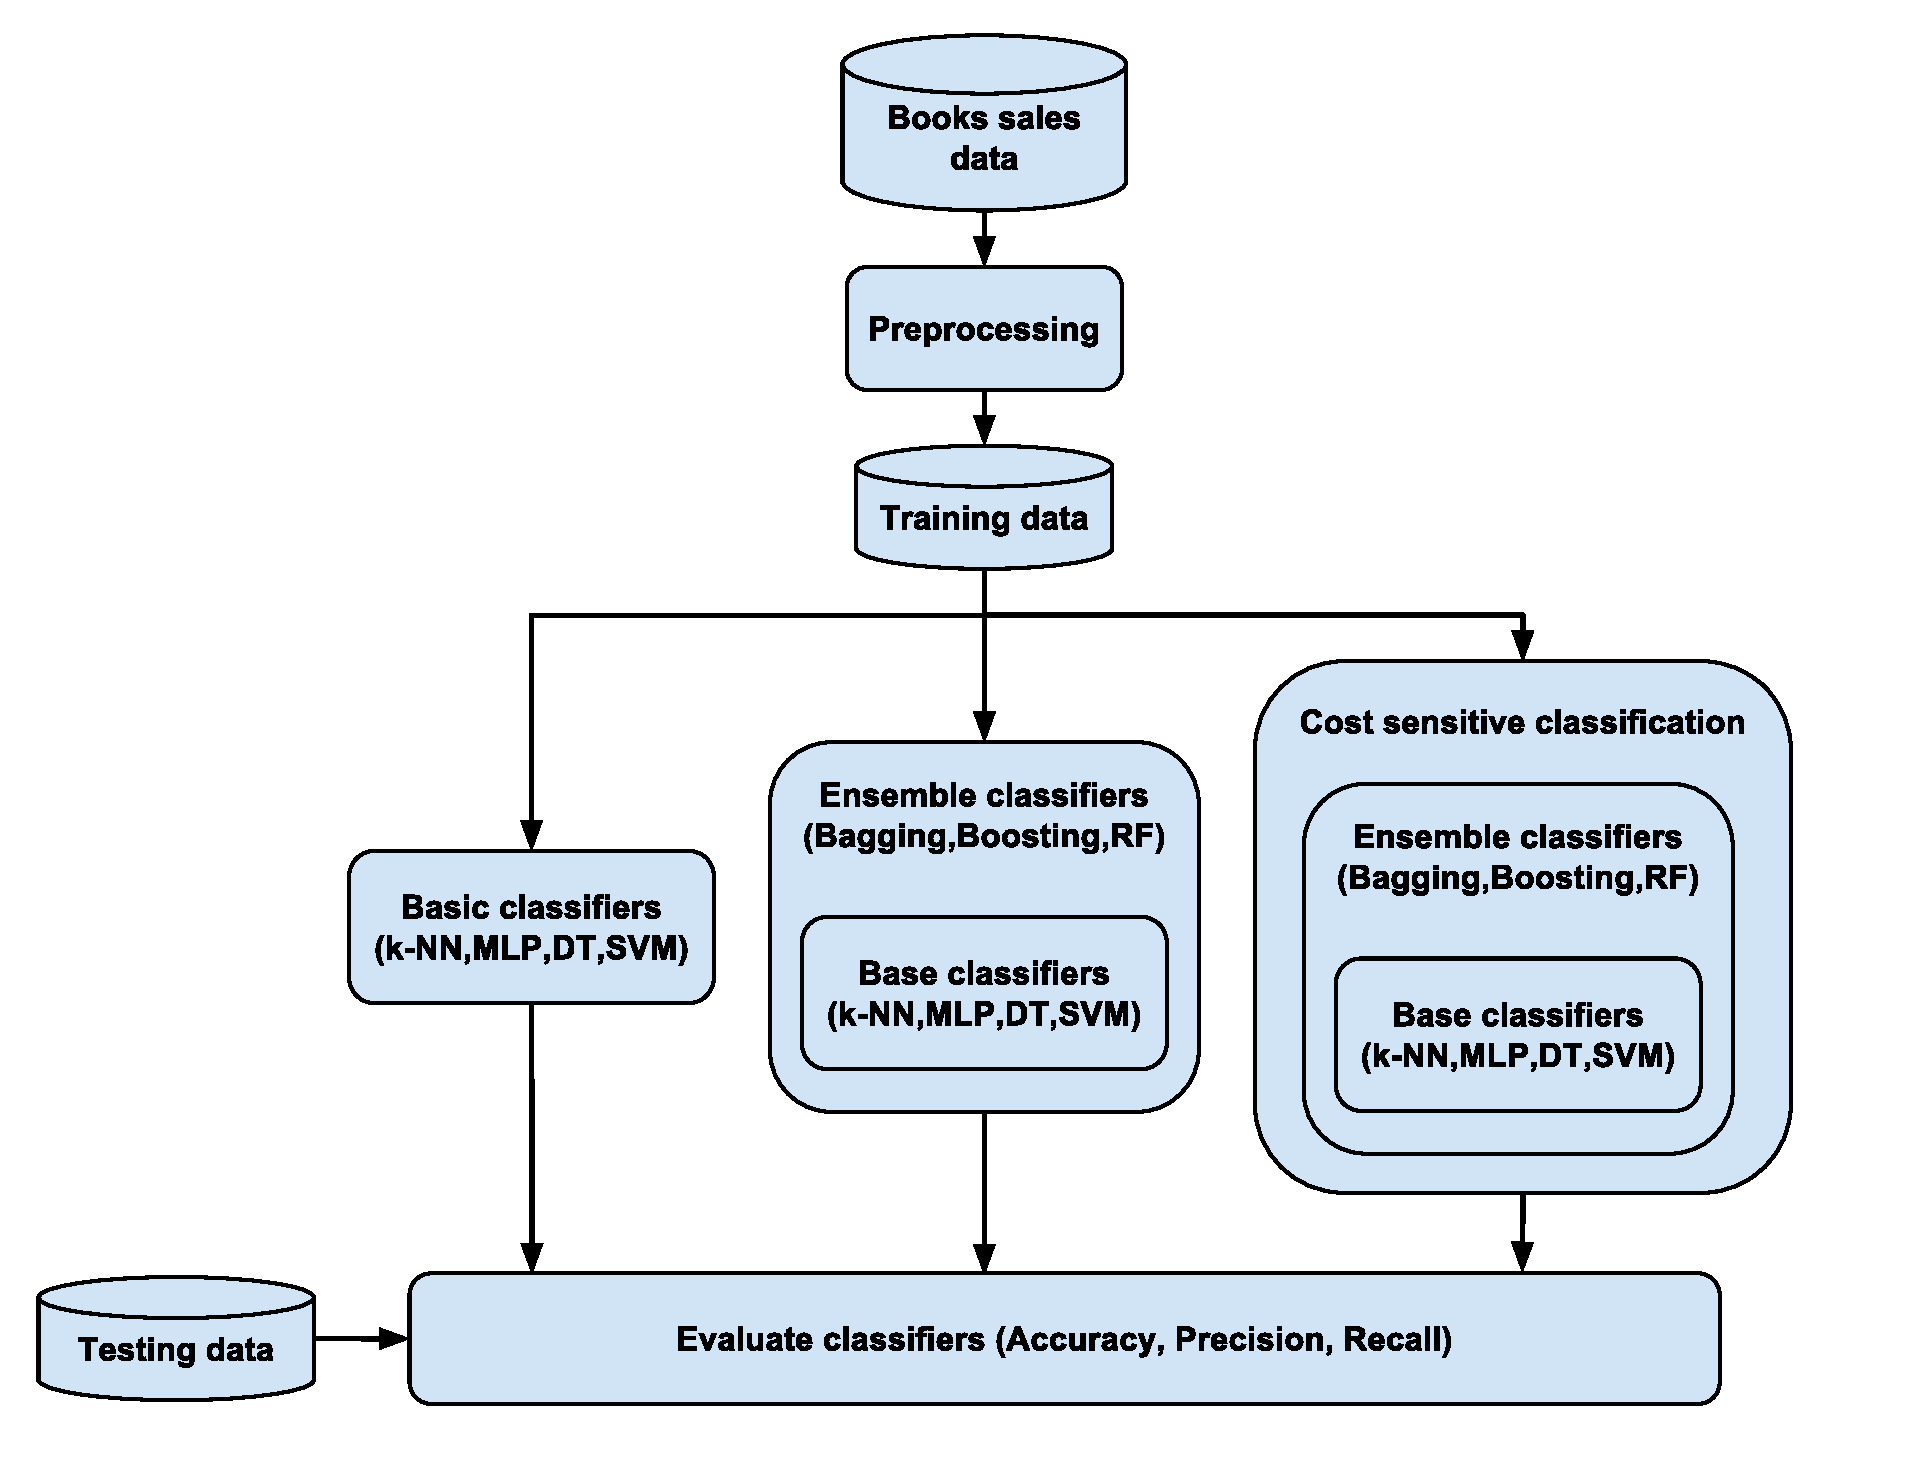
\includegraphics[scale=0.40]{books_methodology}
\end{center}
\caption{Proposed methodology.}
\label{fig:methodology}
\end{figure*}
% Antonio - I like this figure, however, it seems on it that the results of the basic classifier are used as 'starting point' of the ensembles, and the results of these methods are used in the cost sensitive classification... is this correct? Otherwise, maybe we should change the design of the figure. ;D
% Hossam: I have changed the figure as Antonio suggested ;)
% Antonio - It is better now, however, is the evaluation the last stage of the methodology? Won't we choose the best approach based on the results? Won't we compose an useful tool with it as in previous paper? I mean a decision tree or so. ;D

%*******************************************************************************
%										MATERIALS AND METHOD
%*******************************************************************************
\section{Materials and methods}
\label{sec:materials}


%-------------------------- BASIC CLASSIFIERS --------------------------
\subsection{Basic classifiers}
\label{subsec:classifiers}

In order to show the need for more intelligent and complex classification models, basic and more common models are experimented and applied first. 
\begin{itemize}

\item \textbf{$k$-Nearest Neighbors ($k$-NN)}
The kNN \cite{Aha1991,Mitchell1997} method is an instance-based classifier in 
which unknown patterns/instances are classified by relating them to the labelled ones, using a distance measure or function, usually Euclidean or Minkowsky distances.

The algorithm is based on the idea that two patterns with a high distance between them are less likely to belong to the same class than two close ones.

In the simplest approach, for every unknown instance to classify, the algorithm finds its nearest neighbour (in the patterns space), and assigns the class of that neighbour to the unknown pattern.
However, it is more common to apply a more robust approach, in which $k$ neighbours are located, and thus, assigning the majority class of these instances to the unclassified pattern.

\item \textbf{Naive Bayes classifier (NB)}

This is a type of probabilistic classifier, based on the Bayes' Theorem \cite{AI-book_Bayes}, which considers a \textit{naive} (or strong) independence between the variables of the samples to be classified.

It is normally used as a baseline for comparison, because it usually yields competitive results in low computational time. Moreover, naive Bayes classifier shows a very good performance when there is considered a supervised training stage.

This method has a very good scalability, requiring a linear number of parameters to work, depending on the number of variables of the problem. These parameters are the mean and standard deviations of the variables of every class.
Thus, it just evaluates closed-form expressions, not needing to iterate to refine the solutions as most of methods do.


\item \textbf{J48 - Decision Trees (DT)}

This method is an implementation of the C4.5 classifier, which generates the so-called \textit{decision trees}. It was introduced in 1993 by Quinlan \cite{Quinlan1993} as an extension of the ID3 algorithm \cite{Mitchell1997}. 

The algorithm builds a decision tree using the attributes of the input patterns as nodes and considering its values for defining a decision in that node. Thus, for each node, the best attribute for splitting the training set is selected. The criteria for choosing one attribute is based on the difference of entropy (normalized information gain) obtained by every possible division. The one which yields the highest information gain is chosen as the best. This process is repeated for the subsequent data subsets, building subtrees. Normally, the decision tree is iteratively refined (or pruned) to maximize these gains and to avoid useless subtrees.


\item \textbf{Multilayer Perceptron Neural Network (MLP)}

It is an artificial neural network generally used for classification or 
approximation/regression problems \cite{Rosenblatt1962,Widrow1990}. It maps the input data onto an appropriate output, as a generalisation of the standard linear perceptron that uses several layers of nodes, called neurons. Each neuron consists of a linear combination of weighted inputs which is passed through a non-linear activation function to produce its output.

Thus, a MLP is able to solve linearly inseparable problems \cite{SteinwenderBitzer2003}. It is normally trained using a supervised learning 
technique called \textit{back-propagation}. This method was proposed by Werbos, Parker and Rumelhart et al. \cite{Werbos1974,Parker1985,Rumelhart1985}, and consists in updating the weights of the output layer neurons according to the obtained erroneous output. Then, the weights are updated inversely up to the input layer.
There are normally two hidden layers, as some works \cite{Lippmann1987,Bishop1996} demonstrated to be enough to 
create classifying regions of any kind.


\item \textbf{Support Vector Machines (SVM)}
SVM \cite{Cortes1995,Shevade2000} is a method which applies statistical learning theory. In classification problems, the algorithm searches for an optimal hyperplane that separates two classes, maximising the margin between them. 
This hyperplane is defined by a subset of training set samples, called support vectors.

This method is highly robust and reliable even if the space is highly dimensional and the problem is not linearly separable.

SVM has been successfully applied in forecasting and classification problems \cite{Cao2003,MinSVM05,Jari2008}.


\end{itemize}



%-------------------------- ENSEMBLE CLASSIFIERS --------------------------
\subsection{Ensemble classifiers}
\label{subsec:ensembles}

The basic idea of ensemble classification is to train a set of base classifiers and then to combine their prediction using some combination scheme in a hope that the combined prediction will be better than the separated predictions. Empirically, ensemble learners tend to outperform their base members due to the significantly better generalization ability of the ensemble. This is because ensemble learners can reduce the the bias and variance problems of the base learning algorithms \cite{dietterich2002ensemble}. In the following, we describe the most popular ensemble methods: Bagging, Boosting and Random Forests.

\begin{itemize}
\item \textbf{Bagging}: 
It is also called \textit{Bootstrap aggregating} is an ensemble meta-algorithm introduced in \cite{B1996}. Bagging works by training base classifiers (usually decision tree classifiers) based on generated new datasets from the original training dataset. The new generated datasets are drawn randomly with replacement in a size almost equal to the original dataset. 
% Antonio - I cannot understand this sentence (upper one). :/
The final classifier's output is based on aggregating the base classifiers by taking a majority or weighted vote.


\item \textbf{Boosting}: 
It is an ensemble classification algorithm which was firstly proposed in \cite{schapire1990strength}. Boosting is founded on the idea that a set of weak classifiers can create a stronger one. In this work we adopt a powerful a variation of boosting called \textit{Adaptive Boosting} or ``AdaBoost'' for short \cite{FS1997}. AdaBoost operates on a training dataset ${(x_{1},y_{1}),...,(x_{m},y_{m})}$ where each $x_{i}$ is a set of inputs belonging to some domain $X$ and each $y_{i}$ belongs to some label $Y$ assuming $Y$ is a binary class set $\{+1,-1\}$. 


During the learning process, AdaBoost modifies the dataset by weighting its samples. These weights are updated every time a new classifier is trained to increase the focus 
% Antonio - what is the focus here?
on the difficult data instances. Consequently, the final generated classifier is a weighted combination of all trained base classifiers. According to many previous works, 
% Antonio - if you say this, you must add some references. ;P
AdaBoost is not affected 
% Antonio - 'is not affected by' -> 'avoids'?
by overfitting and it can outperform many other state-of-the-art classification techniques.


\item \textbf{Random Forest}:
This method is based on the construction of a set of decision trees using a stochastic process over the basis of C4.5 algorithm. It was proposed by Breiman in \cite{Breiman2001} and aims to create independent and uncorrelated trees based on different and random input vectors, following the same distribution. 
The result is the average of the generated trees during the process.

% Antonio - we should improve a bit this description to do it more complete. ;)

\end{itemize}


%*******************************************************************************
%										COST SENSITIVE CLASSIFICATION
%*******************************************************************************
\section{Cost sensitive classification}
\label{sec:cost_sensitive_classification}


%------------------------ COST SENSITIVE LEARNING ------------------------
\subsection{Cost sensitive learning}
\label{subsec:cost_learning}


%------------------------ COST SENSITIVE CLASSIFICATION ------------------------
\subsection{Cost sensitive classification}
\label{subsec:cost_classification}


%*******************************************************************************
%										DATASET
%*******************************************************************************
\section{Dataset description}
\label{sec:dataset}


The obtained dataset contains collected information about 6083
different books produced by 209 publishers. Each book or pattern in
the dataset is represented by 10 features, listed in Table
\ref{tabla:params_pre_sales}. 
%
\begin{table*}
\caption{Pre-sales features and Sales level(Output class). } 
\label{tabla:params_pre_sales}
\begin{center}
\begin{tabular}{|c|l|l|c|c|}
\hline 
No. & Feature Name & Variable & Type & In/Out\\
\hline 
1 & retail price (when launched) & \texttt{ret\_price} & numerical & input\\
2 & main subject (code) & \texttt{subject1} & numerical & input\\
3 & bookbinding (code) & \texttt{binding} & categorical & input\\
4 & gifts (promotional books) & \texttt{gifts} & numerical & input\\
5 & units distributed as novelty & \texttt{distrib\_novelty} & numerical & input\\
6 & total number of points of sale & \texttt{tot\_points\_sale} & numerical & input\\
7 & total number of points of sale (1st year) & \texttt{tot\_points\_sale\_1st\_year} & numerical & input\\
8 & weeks on sale & \texttt{weeks\_sale} & numerical & input\\
9 & print run & \texttt{print\_run} & numerical & input\\
\hline 
\hline
10 & Sales level & \texttt{sales\_level} & categorical & output\\
\hline 
\end{tabular}
\end{center}
\end{table*}


The output variable related to the total amount of sales is a
categorical variable which represent the level of the quantity sold
for a given book. We have defined four categories to
represent these levels: \textit{Low (L)}, \textit{Medium (M)},
\textit{High (H)}, and \textit{Very High (VH)}. Table \ref{table:freq}
shows the ranges of total sales that correspond to each category along
with the number of sold books that fall in. The discretization of the
volume of sales was conducted by an expert in the domain of editorial
management business, who defined the four categories. They are also
adapted to the Spanish market. The first level, 60, corresponds to the
first quartile in the book sales distribution: 25\% of books sell less
than 60 copies. The second has been established at the typical print
run in the Spanish market, which is 300 copies, including not only
books for sale, but also books sent as a gift, to display or for
reviewers. 1000 books would be considered a decently selling book with
several print runs; second print run will depend on how fast the first
one sales, but could typically be 500 to 1000 new copies. Anything
selling more than 1000 copies will sell extremely well, with only 60
books reaching more than 5000 physical copies sold in the data set we
used. These sales levels will have to be adjusted to particular
markets using the same methodology we have used here, although a good
rule of thumb would be, after examining the initial data set and the
distribution of sales among different books, to choose the 4 quartiles
or 3 terciles and split the top one giving the ``very high'' category
to the books in the top decile. 

Table \ref{table:freq} reveal more information about the nature of the
dataset. Please note that most of the investigated books are
categorized as Low and Medium %once again, unify typography
levels forming 26.8\% and 36.4\% of the dataset, respectively. High
volumes of sold books that range from 301 up to 1000 are categorized
as High volume of sales and form 24\% of the dataset. On the other
hand, books that achieved more than 1000 sold copies are categorized
as Very High and they form around 12.8\% of the dataset. Our focus in
this study is to identify the more profitable categories which are
High and Very High. However, since the latter category is much smaller
than the other ones, we can describe our dataset as imbalanced which
makes the problem of identifying this category harder and more
challenging. 


\begin{table*}[ht]
\caption{Categories corresponding to total sales }
\centering{}%
\begin{tabular}{|c|c|c|c|}
\hline 
Category & Range of total sales & Number of books & Ratio\tabularnewline
\hline 
\hline 
Low & 0-60 & 1631 & 26.8\%\tabularnewline
\hline 
Medium & 61-300 & 2212 & 36.4\%\tabularnewline
\hline 
High & 301-1000 & 1460 & 24\%\tabularnewline
\hline 
Very High & $>$1000 & 780 & 12.8\%\tabularnewline
\hline 
\end{tabular}
\label{table:freq}
\end{table*}


%*******************************************************************************
%										EVALUATION MEASUREMENTS
%*******************************************************************************
\section{Evaluation measurements}
\label{sec:eval_measures}

To evaluate the developed classification models, first, we refer the confusion matrix shown in Table \ref{fig:confusionmatrix} which is considered as a basic source for evaluating any binary classification model. In our case which is a multiclass prediction problem, this matrix can be expanded with a row and column for each class to evaluate the multiclass classification models. Three measurements are used to evaluate the applied classifiers: accuracy rate, precision and recall. The accuracy rate simply measures the total number of correctly classified instances over the total number of instances $N$ as shown in Equation \ref{equation:acc}.

Precision is the ratio of the correctly classified instances as $i$ to the number of instances classified as $i$. On the other side, recall is the ratio of the correctly classified instances as $i$ to the number of actual $i$ instances. Precision and recall are given in Equation \ref{equation:precision} and \ref{equation:recall}, respectively.


\begin{figure*}[ht]
\begin{center}
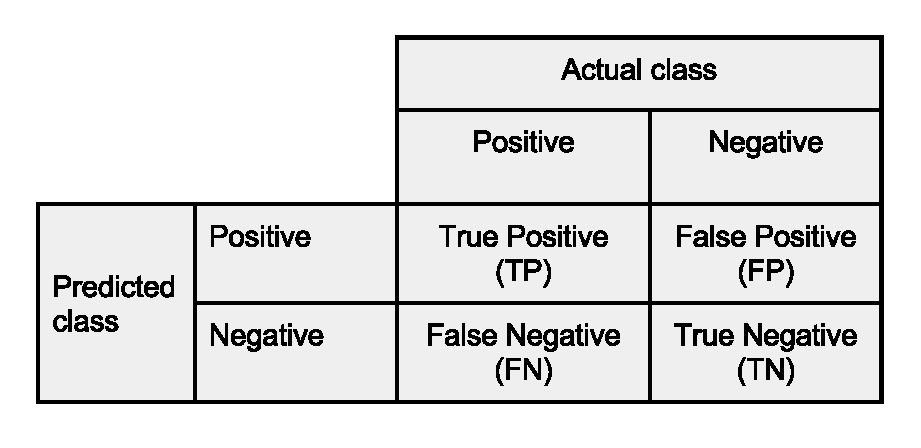
\includegraphics[scale=0.50]{Confusion-matrix}
\end{center}
\caption{Basic confusion matrix.}
\label{fig:confusionmatrix}
\end{figure*}

\begin{equation}
Accuracy=\frac{\sum_{i}C_{ii}}{N}
\label{equation:acc}
\end{equation}


\begin{equation}
Precision_{i}=\frac{C_{ii}}{\sum_{j}C_{ij}}
\label{equation:precision}
\end{equation}


\begin{equation}
Recall_{i}=\frac{C_{ii}}{\sum_{j}C_{ji}}
\label{equation:recall}
\end{equation}

\begin{figure*}[ht]
\begin{center}
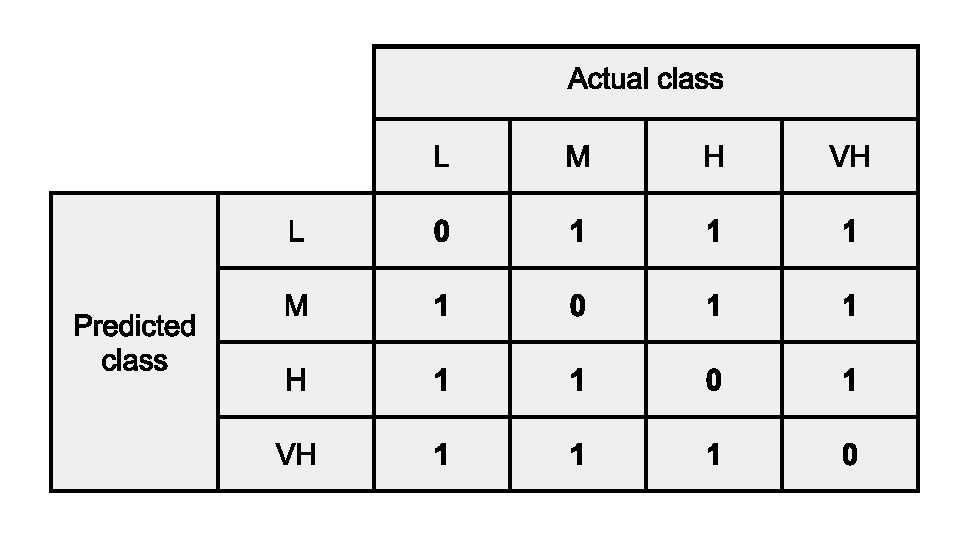
\includegraphics[scale=0.40]{Confusion-matrix-multiclass-default}
\end{center}
\caption{Default cost matrix.}
\label{fig:Default_cost_matrix}
\end{figure*}




\begin{table}
\caption{Cost matrices for three different scenarios}
\centering{}%
\begin{tabular}{|c|c|c|c|c|c|c|c|c|c|c|c|c|c|c|c|}
\hline 
\multicolumn{2}{|c|}{} & \multicolumn{14}{c|}{Actual}\tabularnewline
\hline 
\multicolumn{2}{|c|}{} & \multicolumn{4}{c|}{Cost matrix 1} & \multirow{6}{*}{} & \multicolumn{4}{c|}{Cost matrix 2} & \multirow{6}{*}{} & \multicolumn{4}{c|}{Cost matrix 3}\tabularnewline
\cline{1-6} \cline{8-11} \cline{13-16} 
\multicolumn{2}{|c|}{} & L & M & H & VH &  & L & M & H & VH &  & L & M & H & VH\tabularnewline
\cline{1-6} \cline{8-11} \cline{13-16} 
\multirow{4}{*}{Predicted} & L & 0 & 1 & 2 & 3 &  & 0 & 1 & 2 & 3 &  & 0 & 1 & 2 & 3\tabularnewline
\cline{2-6} \cline{8-11} \cline{13-16} 
 & M & 5 & 0 & 1 & 2 &  & 10 & 0 & 1 & 2 &  & 15 & 0 & 1 & 2\tabularnewline
\cline{2-6} \cline{8-11} \cline{13-16} 
 & H & 10 & 5 & 0 & 1 &  & 20 & 10 & 0 & 1 &  & 30 & 15 & 0 & 1\tabularnewline
\cline{2-6} \cline{8-11} \cline{13-16} 
 & VH & 15 & 10 & 5 & 0 &  & 30 & 20 & 10 & 0 &  & 45 & 30 & 15 & 0\tabularnewline
\hline 
\end{tabular}
\end{table}


%*******************************************************************************
%										EXPERIMENTS AND RESULTS
%*******************************************************************************
\section{Experiments and results}
\label{sec:experiments_results}

%This is just the first step of the experiments
% This table shows the average results of 10X10-folds experiments of the basic classifiers.
% It is impossible to calculate directly the average Precision and Recall for each class for multiclass problems in Weka Experimenter. So I have written a bash script to generate the row predictions utilizing Weka 3.9 developers version. Then I wrote another Python script to process these predicitons and calculate the precision and recall measurements as listed in this table.

In all experiments, 10-folds cross validation methodology is applied for training and testing the developed classifiers. Moreover, in order to generate statistically reliable results, the 10-fold cross validation is repeated 10 times with different partitioning seeds then the average and standard deviation are calculated for each evaluation metric.

In the first stage of the experiments the basic classifiers k-NN, NB, MLP, J48 and SVM are applied for predicting the sales level. The performance of some classifiers is highly affected by the initial values of their parameters. For this reason, initial experiment were conducted to tune the parameters of k-NN, SVM and MLP. For k-NN the best classification results were obtained with k=1. For SVM, a rough grid search was used, the value for the cost $C$ is set to 50 and $\gamma$  to 0.01. For MLP, the number of hidden neurons is set to (number of features+ number of output classes)/2.


The developed classifiers are assessed by measuring their accuracy and the precision and recall of each class label. Evaluation measures for all classifiers are shown in Table \ref{table:basic_classifiers}. 

\begin{table*}
\caption{Classification results using basic classifiers (without print-run)}
\centering{}%
\begin{tabular}{|c|c|c|c|c|c|}
\hline 
 & kNN  & NB  & J48  & MLP  & SVM\tabularnewline
\hline 
\hline 
$Accuracy$  & 0.69$\pm$0.0026 & 0.67$\pm$0.0008 & 0.7$\pm$0.004 & 0.71$\pm$0.0027 & 0.67$\pm$0.0012\tabularnewline
\hline 
\hline 
$Recall_{L}$  & 0.75$\pm$0.0044 & 0.86$\pm$0.0013 & 0.79$\pm$0.0071 & 0.78$\pm$0.0222 & 0.59$\pm$0.0035\tabularnewline
\hline 
$Precision_{L}$  & 0.78$\pm$0.003 & 0.73$\pm$0.0017 & 0.8$\pm$0.0049 & 0.8$\pm$0.0173 & 0.84$\pm$0.0025\tabularnewline
\hline 
\hline 
$Recall_{M}$  & 0.74$\pm$0.0034 & 0.66$\pm$0.0024 & 0.7$\pm$0.0072 & 0.71$\pm$0.0129 & 0.82$\pm$0.002\tabularnewline
\hline 
$Precision_{M}$  & 0.65$\pm$0.003 & 0.64$\pm$0.0007 & 0.68$\pm$0.0079 & 0.69$\pm$0.007 & 0.59$\pm$0.0012\tabularnewline
\hline 
\hline 
$Recall_{H}$  & 0.59$\pm$0.0047 & 0.53$\pm$0.0022 & 0.6$\pm$0.0099 & 0.65$\pm$0.0346 & 0.55$\pm$0.0016\tabularnewline
\hline 
$Precision_{H}$  & 0.62$\pm$0.0037 & 0.58$\pm$0.0017 & 0.62$\pm$0.0058 & 0.62$\pm$0.0109 & 0.63$\pm$0.0012\tabularnewline
\hline 
\hline 
$Recall_{VH}$  & 0.6$\pm$0.0073 & 0.53$\pm$0.003 & 0.72$\pm$0.0086 & 0.68$\pm$0.0336 & 0.61$\pm$0.0012\tabularnewline
\hline 
$Precision_{VH}$  & 0.79$\pm$0.0071 & 0.81$\pm$0.0032 & 0.74$\pm$0.0072 & 0.77$\pm$0.0212 & 0.78$\pm$0.0028\tabularnewline
\hline 
\end{tabular}
\label{table:basic_classifiers}
\end{table*}

It can be noticed that all classifiers have obtained very close accuracy ratios with a slight advantage for the MLP network with 71\% accuracy. In general, accuracy rates don't give an insight on how the classifier performs regarding each class. Therefore, precision and recall rates are examined for each class. Precision and recall values in Table \ref{table:basic_classifiers} show that J48 classifier achieved the highest recall value of 72\% for (VH) class with 74\% precision. The second best classifier for this important class is MLP with 68\% recall and 77\% precision. Having a look at the second important class which is (H), we can see that MLP has the highest recall with 65\% and a precision of 62\%. J48 comes second for the (H) class with a slight decrease in the recall value.

In the next stage of the experiments, the ensemble classifiers (i.e. RF, Bagging and AdaBoost) are applied and evaluated. For Bagging and AdaBoost, the base classifier is selected to be the J48 decision tree algorithm. This selection is for three reasons: first, the J48 algorithm achieved very competitive evaluation results in the previous phase. Second, J48 is much faster as a learning algorithm compared to the MLP network which was the second candidate. Third, tree induction algorithms are good candidates as base classifiers in bagging and boosting because support diversity among the learners. It is well known that tree induction algorithms are relatively unstable (i.e. weak) base learners, meaning that small changes in the training data lead to big changes in the developed models. Besides the selection of the base classifier, the effect of the number of iterations is experimented in RF, Bagging and AdaBoost as shown in Figures \ref{fig:PerformanceRF}, \ref{fig:PerformanceBagging} and \ref{fig:PerformanceAdaboost}, respectively. Highest prediction rates are obtained at 60 iterations. The best obtained results for these ensemble classifiers are shown in Table \ref{table:ensemble_classifiers}. It can be seen that all ensemble classifiers achieved higher accuracy rates compared to J48 from the previous stage, achieving around 74\% with approximately 4\% improvement. Inspecting the obtained results for VH class, we can notice that although the recall of the VH hasn't improved much compared to J48, the precision has remarkably increased from 74\% to 81.6\%, 80.8\% and 79.3\% for RF, Adaboost and Bagging, respectively. For the H class, there was an improvement for both measurements, recall and precision. RF and Adaboost achieved approximately 68\% and 67\% for recall and precision, while Bagging achieved 67\% and 66\%, respectively. Also, it can be noticed that there is an improvement in general for the other classes, M and L.


\begin{figure*}

\centerline{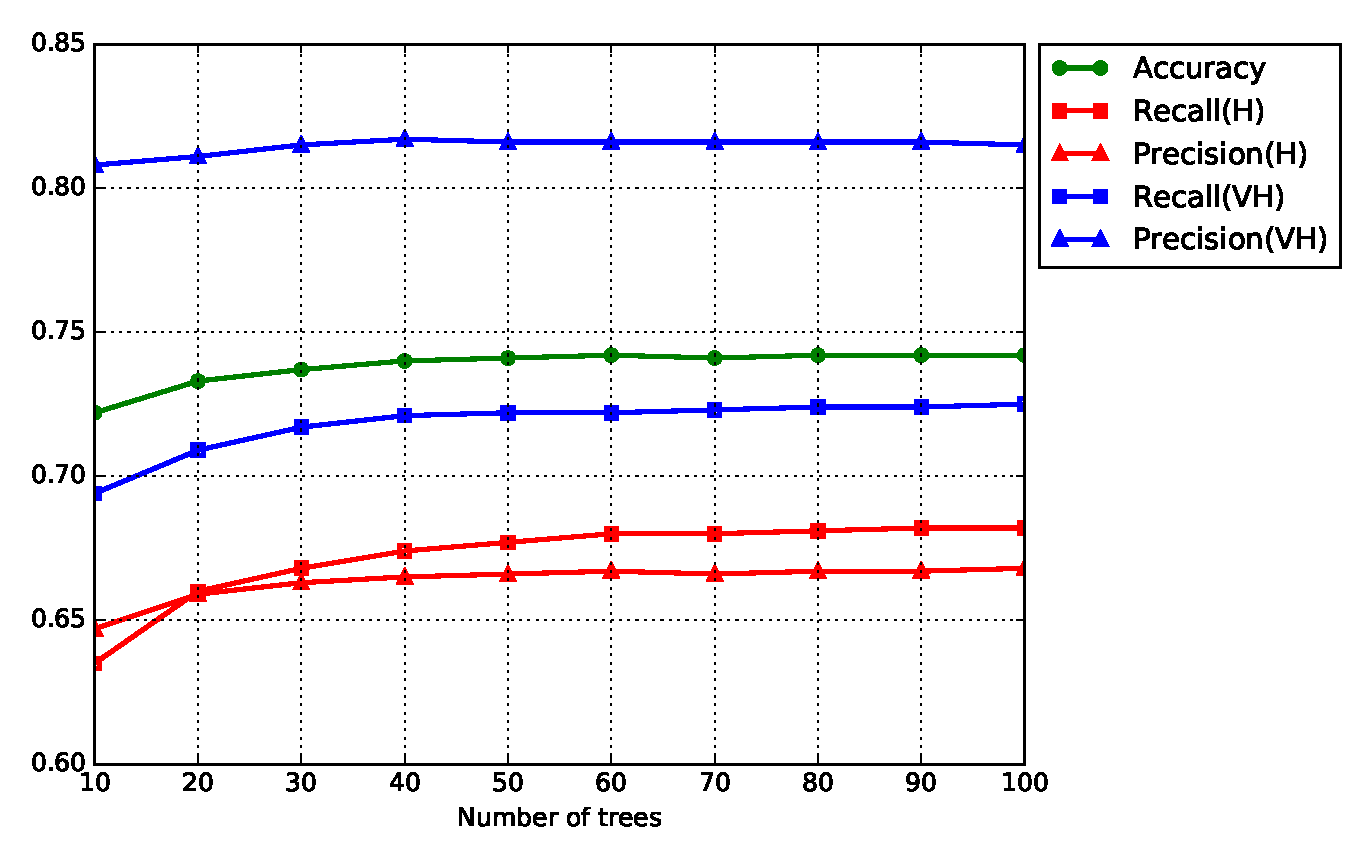
\includegraphics[scale=0.46]{RF}}

\caption{Performance of RF classifier over different number of trees.}
\label{fig:PerformanceRF}
\end{figure*}

\begin{figure*}
\centerline{
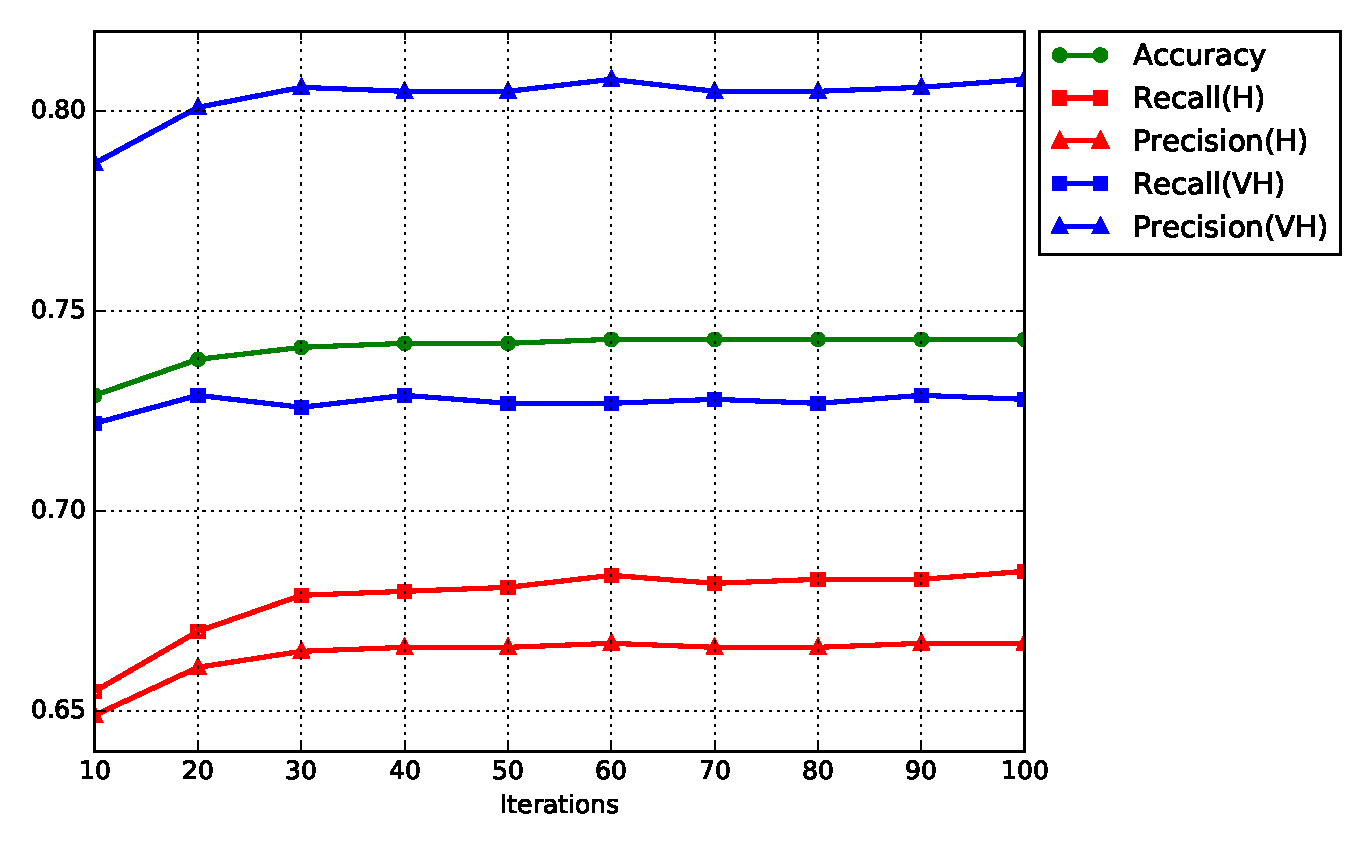
\includegraphics[scale=0.46]{Bagging}}

\caption{Performance of Bagging classifier over different number of iterations.}
\label{fig:PerformanceBagging}
\end{figure*}

\begin{figure*}
\centerline{
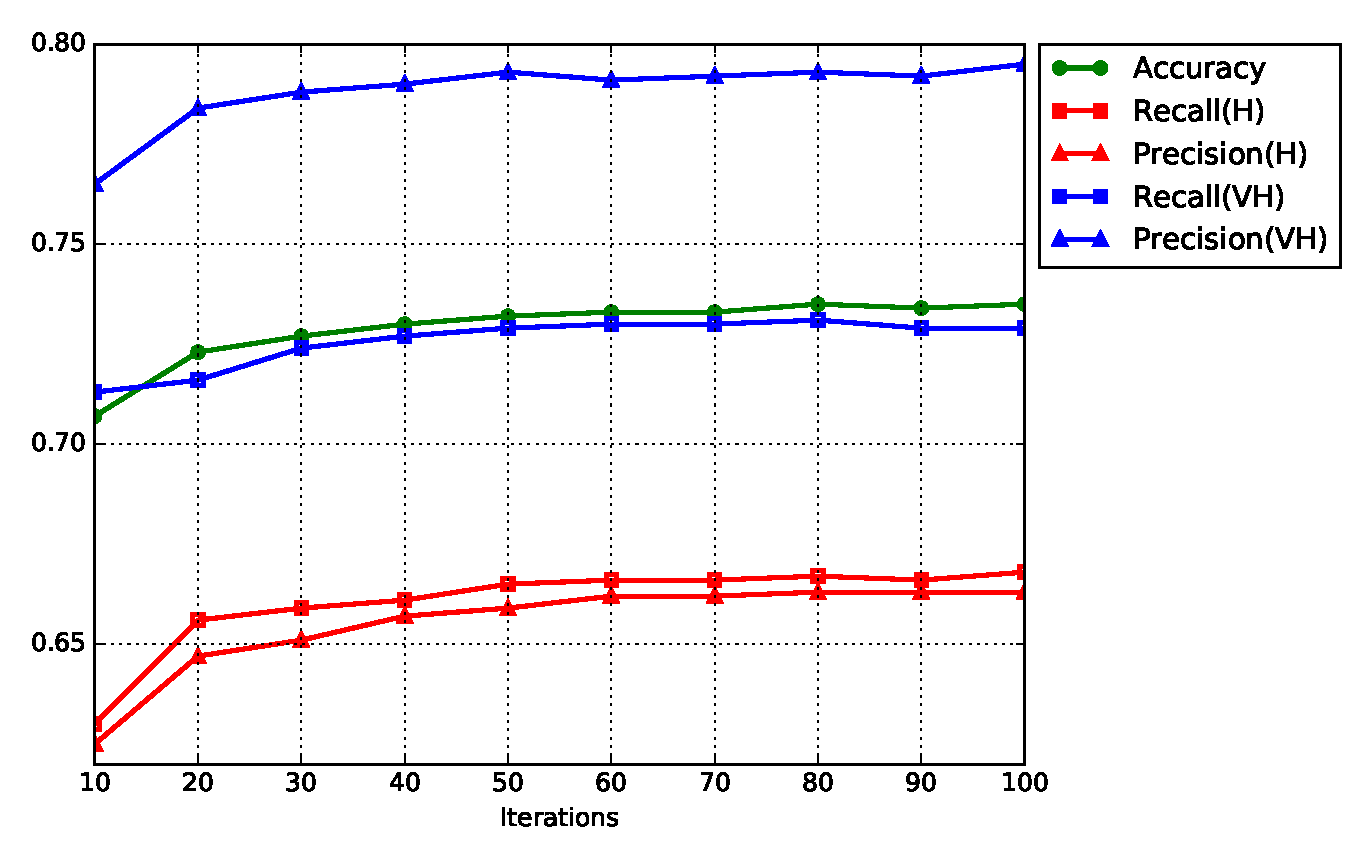
\includegraphics[scale=0.46]{Adaboost}
}
\caption{Performance of Adaboost classifier over different number of iterations.}
\label{fig:PerformanceAdaboost}
\end{figure*}


\begin{table*}
\caption{Classification results using ensemble classifiers (RF, AdaBoost and Bagging)}
\centering{}%
\begin{tabular}{|c|c|c|c|}
\hline 
 & RF  &  AdaBoost &  Bagging \tabularnewline
\hline 
 \hline $Accuracy$ & 0.741 $\pm$ 0.002 & 0.743 $\pm$ 0.0023 & 0.735 $\pm$ 0.0022 \tabularnewline 
 \hline 
 \hline $Recall_{L}$ & 0.796 $\pm$ 0.0038 & 0.793 $\pm$ 0.0038 & 0.792 $\pm$ 0.0048 \tabularnewline 
 \hline $Precision_{L}$ & 0.823 $\pm$ 0.0035 & 0.827 $\pm$ 0.0032 & 0.814 $\pm$ 0.0043 \tabularnewline 
 \hline 
 \hline $Recall_{M}$ & 0.748 $\pm$ 0.0033 & 0.75 $\pm$ 0.0029 & 0.738 $\pm$ 0.0038 \tabularnewline 
 \hline $Precision_{M}$ & 0.712 $\pm$ 0.0026 & 0.716 $\pm$ 0.0032 & 0.707 $\pm$ 0.004 \tabularnewline 
 \hline 
 \hline $Recall_{H}$ & 0.68 $\pm$ 0.0073 & 0.684 $\pm$ 0.0051 & 0.667 $\pm$ 0.0065 \tabularnewline 
 \hline $Precision_{H}$ & 0.666 $\pm$ 0.0037 & 0.667 $\pm$ 0.0029 & 0.663 $\pm$ 0.004 \tabularnewline 
 \hline 
 \hline $Recall_{VH}$ & 0.723 $\pm$ 0.0054 & 0.727 $\pm$ 0.0041 & 0.731 $\pm$ 0.0057 \tabularnewline 
 \hline $Precision_{VH}$ & 0.816 $\pm$ 0.0051 & 0.808 $\pm$ 0.0056 & 0.793 $\pm$ 0.0069 \tabularnewline 
\hline 
\end{tabular}
\label{table:ensemble_classifiers}
\end{table*}

%*******************************************************************************
%										CONCLUSIONS AND FUTURE WORK
%*******************************************************************************
\section{Conclusions and Future Work}
\label{sec:conclusions_future_work}





%********************************************************************************
\section*{Acknowledgements}

This work has been supported in part by projects PreTEL (PRM
Consultores - Trevenque S.L.), TIN2014-56494-C4-3-P and TEC2015-68752
(Spanish Ministry of Economy and Competitiveness and FEDER), and
PROY-PP2015-06 (Plan Propio 2015, funded by the University of Granada,
Spain).
% Is still this last grant running? 



%********************************************************************************
\bibliographystyle{elsarticle-num}
\bibliography{refs}

%----------------------------------------------------------------------

\end{document}
